\smalltitle{سوال 4}
\begin{enumerate}
    \item در ابتدا برای کشیدن جدول ستون‌های مورد نیاز را مشخص می‌کنیم.
    چند ستون اول صرفا با توجه به داده‌های سوال بدست می‌آیند. ستون
    \lr{Arrival Time}
    صرفا جمع تمام مقدایر
    \lr{Time Since Last Arrival}
    قبل از آن است.
    زمانی که یک
    \lr{task}
    جدید می‌آید، در ابتدا باید چک کنیم که آیا کارت گرافیک‌ها بی‌کار هستند یا خیر. این موضوع را می‌توان با نگاه
    کردن به
    \lr{Time Task Ends}های
    تسک‌های قبلی بدست آورد. در صورتی که هیچ تسکی وجود نداشت که زمان اتمام آن بعد از زمان رسیدن این تسک جدید بود،
    بدون هیچ گونه صبری تسک وارد کارت گرافیک می‌شود. در غیر این صورت باید به اندازه‌ی
    \lr{Arrival Time}
    منهای ماکسیموم
    \lr{Time Since Last Arrival}
    صبر کنیم. به کمک همین اعداد می‌توان زمان شروع و پایان را نیز مشخص کرد.
    \begin{latin}
        \centering
        \scriptsize
        \begin{tabular}{|c|c|c|c|c|c|c|c|c|c|c|c|}
        \hline
        ID & \makecell{Time\\Since\\Last\\Arrival} & \makecell{Arrival\\Time} & \makecell{GPU 1\\Task Time} & \makecell{GPU 2\\Task Time} & \makecell{Wait\\Time} & \makecell{Time\\Task\\Starts} & \makecell{Time\\Task\\Ends} & \makecell{GPU Picked\\Up Task} & \makecell{Time\\Tasks\\Executes} & \makecell{GPU 1\\Idle} & \makecell{GPU 2\\Idle}\\
        \hline
        1 & - & 0 & 4 & 2 & 0 & 0 & 2 & 2 & 2 & 0 & 0 \\
        \hline
        2 & 3 & 3 & 7 & 9 & 0 & 3 & 10 & 1 & 7 & 3 & 1 \\
        \hline
        3 & 2 & 5 & 5 & 4 & 0 & 5 & 9 & 2 & 4 & 0 & 3 \\
        \hline
        4 & 1 & 6 & 4 & 1 & 3 & 9 & 10 & 2 & 1 & 0 & 0 \\
        \hline
        5 & 2 & 8 & 7 & 9 & 2 & 10 & 17 & 1 & 7 & 0 & 0 \\
        \hline
        6 & 1 & 9 & 8 & 5 & 1 & 10 & 15 & 2 & 5 & 0 & 0 \\
        \hline
        7 & 2 & 11 & 6 & 4 & 4 & 15 & 19 & 2 & 4 & 0 & 0 \\
        \hline
        8 & 1 & 12 & 4 & 8 & 5 & 17 & 21 & 1 & 4 & 0 & 0 \\
        \hline
        9 & 2 & 14 & 5 & 2 & 5 & 19 & 21 & 2 & 2 & 0 & 0 \\
        \hline
        10 & 3 & 17 & 9 & 7 & 4 & 21 & 28 & 2 & 7 & 0 & 0 \\
        \hline
    \end{tabular}
    \end{latin}
    \item \phantom{kir}
    \begin{latin}
    \centering
    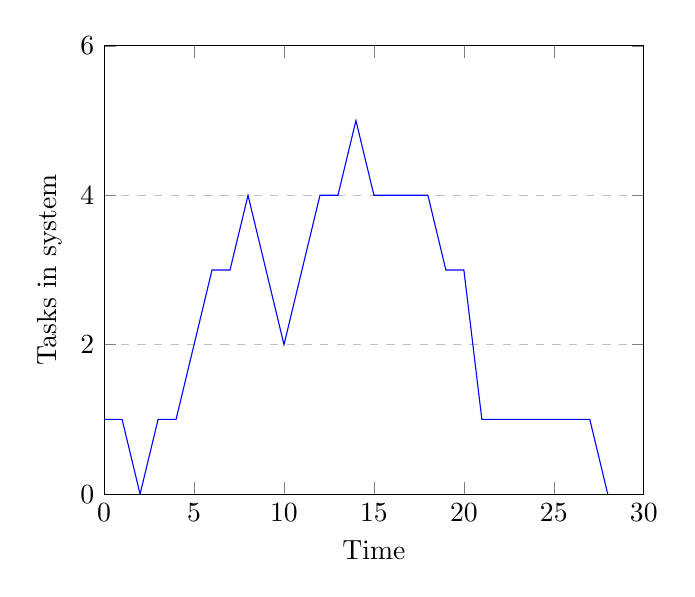
\begin{tikzpicture}
    \begin{axis}[
        xlabel={Time},
        ylabel={Tasks in system},
        xmin=0, xmax=30,
        ymin=0, ymax=6,
        legend pos=north west,
        ymajorgrids=true,
        grid style=dashed,
    ]
    
    \addplot[
        color=blue,
        ]
        coordinates {
        (0,1)(1,1)(2,0)(3,1)(4,1)(5,2)(6,3)(7,3)(8,4)(9,3)(10,2)(11,3)(12,4)(13,4)(14,5)(15,4)(16,4)(17,4)(18,4)(19,3)(20,3)(21,1)(27,1)(28,0)
        };
    \end{axis}
    \end{tikzpicture}
    \end{latin}
    \item \phantom{kir}
    \begin{latin}
    \centering
    \begin{tikzpicture}
    \begin{axis}[
        xlabel={Time},
        ylabel={Queue length},
        xmin=0, xmax=30,
        ymin=0, ymax=6,
        legend pos=north west,
        ymajorgrids=true,
        grid style=dashed,
    ]
    
    \addplot[
        color=blue,
        ]
        coordinates {
        (0,0)(5,0)(6,1)(7,1)(8,2)(9,2)(10,0)(11,1)(12,2)(13,2)(14,3)(15,2)(16,2)(17,2)(18,2)(19,1)(20,1)(21,0)(28,0)
        };
    \end{axis}
    \end{tikzpicture}
    \end{latin}
    \item با توجه به جدول برای کارت گرافیک اول 
    $3 + (28 - 21) = 10$
    و برای کارت گرافیک دوم
    $5 - 2 = 3$
    واحد زمانی
    \item برای هر تسک در جدول نوشته شده است. برای کل تسک‌ها نیز داریم:
    \begin{gather*}
        \frac{3 + 2 + 1 + 4 + 5 + 5 + 4}{10} = 2.4
    \end{gather*}
    \item می‌توان تعداد کارت گرافیک‌ها یا قدرت آن‌ها را بیشتر کرد.
\end{enumerate}